\chapter{ANÁLISIS LÉXICO}
\section{INTRODUCCIÓN}
\subsection{TERMINOLOGÍA}
\begin{itemize}
    \item Token: Categorías léxicas
    \item Buffer:
    \item Lexema: 
    \item Patrón: Plantilla que permite determinar si un objeto pertenece a una clase especifica
    \item Expresión Regular: Modelo matemático usado para reconocer lenguajes regulares
    \item Definición Regular:
    \item Notación Extendida de Expresiones Regulares: 
    \item Diagramas de Transición:
    \item AFN:
    \item AFD:
    \item Conversión de Expresiones Regulares en Autómatas: Algoritmo que recibe una expresión regular y la transforman en un autómata que la reconoce. 
    \item LEX: 
    \item Diseño de generadores de análisis léxico: 
\end{itemize}


\section{LENGUAJES Y LENGUAJES REGULARES}
\subsection{Especificaciones del vocabulario}
Alfabeto: $\Sigma = \{a_i\}^{i=n}_{i=1} \quad n \in \mathbb{N}, n \neq 0$\\
Ejemplos:
\begin{itemize}
    \item $\Sigma = \{0,1\}$
    \item $\Sigma = \{\alpha\}$
    \item $\Sigma = \text{ASCII}$
\end{itemize}\\
No ejemplos:
\begin{itemize}
    \item $\Sigma = \{a, ab, b\}$
    \item $\Sigma = \emptyset$ 
\end{itemize}

\subsection{Cadenas}
Concatenaciones de símbolos del alfabeto:
\begin{enumerate}
    \item $\Sigma ^ 0 = \{\lambda\} \neq \emptyset$. $\lambda$ simboliza la cadena vacía
    \item $\Sigma ^ 1 = \Sigma$
    \item $\Sigma ^{n+1} = \{as|a\in\Sigma, \wedge, s\in\Sigma^n\}$
\end{enumerate}
Ej:
Dado $\Sigma = \{a,b\}$
\begin{enumerate}
    \item $\Sigma ^ 0 = \{\lambda\}$
    \item $\Sigma ^ 1 = \{a,b\}$
    \item $\Sigma ^ 2 = \{aa, ab, ba, bb\}$
    \item $\Sigma ^ 1 \cup \Sigma ^ 2 = \{a, b, aa, ab, ba, bb\}$
\end{enumerate}
Hay 2 conjuntos particulares:\\
\begin{align*}
    \Sigma^+ &= \bigcup^{+\infty}_{n = 1}\Sigma^n\\
    \Sigma^* &= \bigcup^{+\infty}_{n = 0}\Sigma^n = \Sigma^+\cup\{\lambda\} \\
\end{align*}

$\Sigma^+$ se llama Cerradura positiva.\\
$\Sigma^*$ se llama Cerradura de Kleene.\\

Un vocabulario se define como:
\[
    \Sigma^*_v \subseteq \Sigma^*
\]

Se caracteriza por que sus palabras tienen un significado. En el caso general los significados de las palabras tienen un único significado, pero en lenguajes mas complejos pueden tener múltiples acepciones o significados.

Si se tiene un alfabeto $\Sigma^*$ se pueden construir 2 subconjuntos:
\begin{itemize}
    \item $G$: palabras Generales del lenguaje. No requieren un diccionario. Son los nombres. 
    \item $P$: palabras Propias del lenguaje, como los while, if, for, etc. Solo tienen un significado. Usualmente tienen un significado, por eso no hay necesidad de que halla un diccionario para dar todos los posibles significados de una palabra como ocurre en el español o ingles.
    
\end{itemize}
$\Sigma^*_v=P\cup G$\\

\subsubsection{Conceptos sobre cadenas}\\
Sea $s \in \Sigma^*$
\begin{itemize}
\item Prefijo: 
    \begin{align*}
        & s = s_1 s_2,\quad s_i \in \Sigma^*\\
        & s_1 \text{ es un prefijo}
    \end{align*}
    
\item Subfijo: 
    \begin{align*}
        & s = s_1 s_2 s_3,\quad s_i \in \Sigma^*\\
        & s_3 \text{ es un subfijo}
    \end{align*}
\item Sub-cadena: 
    \begin{align*}
        & s = s_1 s_2 s_3,\quad s_i \in \Sigma^*\\
        & s_2 \text{ es una sub-cadena}
    \end{align*}
\item Prefijo, subfijos, sub-cadena ``propios'': no son $\lambda$ ni $s$ en si mismos
\item Sub-secuencia: Cadena formada a partir de $s$ 
\end{itemize} ``borrando'' algunos símbolos de $s$ no necesariamente consecutivos

\subsection{Lenguajes}
Dado $\Sigma$ y $\Sigma^*$ un lenguaje es:
\begin{equation*}
    L \subseteq \Sigma^*
\end{equation*}
Es necesario ademas que las cadenas de $L$ deben estar dotadas de significado.\\
Ejemplos:\\
Sea $\Sigma = \{a, b\}$, $\Sigma^*=\{\lambda, a, b, aa, ab, ba, \dots\}$
\begin{enumerate}
    \item $L=\{\}=\emptyset$
    \item $L = \Sigma^*$
    \item $L = \Sigma$
    \item $L = \{aa, bb\}$
\end{enumerate}
\subsubsection{Operaciones sobre lenguajes}
Dado $\Sigma$, y $L_1, L_2, \dots, L_i, \dots$
\begin{itemize}
    \item Unión: 
    \begin{equation*}
        L = L_1\cup L_2 = \{w|w\in L_1, \lor, w\in L_2\}
    \end{equation*}
    \item Concatenación: 
    \begin{equation*}
        L = L_1 L_2 = \{w|w\in L_1, \land, w\in L_2\}
    \end{equation*}
    \item Cerradura positiva: 
    \begin{equation*}
        L^+_j = \bigcup^{+\infty}_{i=1}L^i_j
    \end{equation*}
    \item Cerradura de Kleene: 
    \begin{equation*}
        L^*_j = \bigcup^{+\infty}_{i=0}L^i_j
    \end{equation*}
\end{itemize}
\\
Ejemplos:\\\\
Dados $\Sigma = \{a, b\}$, $L_1 = \{aa, ab\}$:
\begin{itemize}
    \item $L^1_1 = \{aa, ab\} = L_1$
    \item $L^2_1 = L_1 L_1 = \{aaaa, aaab, abaa, abab\}$
    \item $L^0_1 = \{\}$
\end{itemize}
\\
Sea $L_1 = \{a,b,c,\dots,z,A,B,C,\dots,Z\}$, $L_2=\{0,1,2,\dots,9\}$:
\begin{itemize}
    \item $L=L_1 \cup L_2$: Letras y números.
    \item $L=L_1 \L_2$: Letra seguido de dígito.
    \item $L=L_1^4$: Cadenas de 4 caracteres.
    \item $L=L_2^+$: Números Naturales. $\mathbb{N}$.
    \item $L=L_1(L_1\cup L_2)^*$: Cadenas que empiezan con letra.
\end{itemize}

\subsubsection{Teorema 1}
Dado $\Sigma$ entonces $\Sigma^*$ es infinito contable.\\
Observación: $\Sigma^*=\{w_i\}_{i \in \mathbb{N}}$

\subsubsection*{Idea de demostración}

Sea 
\begin{equation*}
    \Sigma = \{a_k\}_{k=1}^{k=m}\quad m \in \mathbb{N},\land,m < \infty
\end{equation*}
Entonces es posible asociar cada cadena de $\Sigma^*$ de la siguiente forma:
\begin{align*}
    \lambda &\rightarrow 0\\
    a_1 & \rightarrow 1\\
    a_2 & \rightarrow 2\\
    &\vdots\\
    a_m &\rightarrow m\\
    a_1 a_1 &\rightarrow m + 1\\
    & \vdots \\
\end{align*}

Por lo que se puede definir una función biyectiva entre las cadenas de $\Sigma^*$ y $\mathbb{N}$

\subsubsection{Teorema 2}

Sea:
\begin{align*}
    &\Sigma &&\text{Alfabeto}\\
    &\Sigma^* &&\text{Conjunto de todas las posibles palabras}\\
    &\mathbb{L} &&\text{Conjunto de todos los lenguajes}\\
\end{align*}\\
Entonces $\mathbb{L}$ es infinito incontable.

Observación: $\mathbb{L} = \{L_j\}_{j \in \mathbb{R}}$

\subsection{Lenguajes Regulares}
Son muy útiles para reconocer el vocabulario de un lenguaje de programación. No son medibles con respecto a $\mathbb{L}$.\\
Se definen como:\\
Dado $\Sigma$
\begin{enumerate}
    \item $L=\emptyset$ es un lenguaje regular
    \item $L=\{\lambda\}$ es un lenguaje regular
    \item $L=\{a_i\}, \quad a_i \in \Sigma$ es un lenguaje regular\\
    
\end{enumerate}
Si $L_1$ y $L_2$ son lenguajes regulares entonces
\begin{enumerate}
    \item $L=L_1\cup \L_2$ es un lenguaje regular
    \item $L=L_1 \L_2$ es un lenguaje regular
    \item $L=L_1^*$ es un lenguaje regular
    \item $L=L_1^+$ es un lenguaje regular
\end{enumerate}

Ningún otro lenguaje es un lenguaje regular.\\
Ejemplos:\\
Dado $\Sigma=\{a, b\}$
\begin{itemize}
    \item $L=\{\lambda\}$
    \item $L=\{b\}$
    \item $L=\{ab\}$
    \item $L=\{(ab)^i|i \geq 0\}$
\end{itemize}

\subsubsection*{Distancia de Damerau-Levenshtein}

Sea $X$ un conjunto de elementos o palabras, entonces $d(a, b)$ es la distancia métrica. $d:X\times X \rightarrow \mathbb{R}$.\\
ej: $d(\text{JAVA}, \text{C})$
$d$ cumple:\\

\begin{align*}
    &\forall a,b \in X && \Rightarrow && d(a, b) \geq 0\\
    &\forall a,b \in X && \Rightarrow && d(a, a) = 0\\
    &\forall a,b \in X && \Rightarrow && d(a, b) = d(b, a)\\
    &\forall a,b,c \in X && \Rightarrow && d(a, b) \leq d(a, c) + d(c, b)\\
    &\forall a,b \in X && \Rightarrow && d(a, b) = 0 \Rightarrow a = b\\
\end{align*}

La distancia de Damerau-Levenshtein se define como el número mínimo de operaciones (inserción, eliminación, substitución de caracteres del alfabeto) requeridas para trasformar una palabra en otra.\\
Ej: $d(casa, calle) = ?$
\begin{enumerate}
    \item casa $\rightarrow$ cala (substitución de "s" por "l")
    \item cala $\rightarrow$ calla (inserción de "l" entre "l" y "a")
    \item calla $\rightarrow$ calle (substitución de "a" por "e")
\end{enumerate}

$d(casa, calle) = 3$

\section{EXPRESIONES REGULARES Y AUTÓMATAS}
Permiten reconocer si una cadena pertenece o no pertenece a un lenguaje regular.\\
Se definen como:


\begin{enumerate}
    \item Si $r=\lambda$ entonces $r$ es una expresión regular y $L(r)= L(\lambda)=\{\lambda\}$
    \item Si $r=a_i,\; a_i\in\Sigma$ entonces $r$ es una expresión regular y $L(r)=L(a_i)= \{a_i\}$
\end{enumerate}
Sean $r$ y $s$ expresiones regulares entonces:

\begin{enumerate}
    \item $(r)|(s)$ es una expresión regular y $L((r)|(s))=L(r)\cup L(s)$
    \item $(r)(s)$ es una expresión regular y $L((r)(s))=L(r) L(s)$
    \item $(r)^*$ es una expresión regular y $L((r)^*)=(L(r))^*$
    \item $(r)^+$ es una expresión regular y $L((r)^+)=(L(r))^+$
\end{enumerate}

Ejemplos:\\
Sea $\Sigma =\{a, b\}$

\begin{enumerate}
    \item  $a|b \quad L=\{a, b\}$
    \item  $(a|b)(a|b) \quad L=\{aa, ab, ba, bb\}$
    \item  $a^* \quad L=\{\lambda, a, aa, aaa, \dots\}$
    \item  $(a|b)^* \quad L=\{\lambda, a, b, aa, ab, ba, bb, aaa, \dots\}$
\end{enumerate}

\subsection{Equivalencia}

Sean $r$ y $s$ expresiones regulares. $r$ es equivalente a $s$ si los lenguajes que reconocen son iguales.
\begin{equation*}
    r \Leftrightarrow s \Longleftrightarrow L(r) = L(s) 
\end{equation*}
Ejemplo:\\
\begin{align*}
&r = (a^*b)^*\\
&s = \lambda|(a1b)^*\\
&L(r) = L(s)
\end{align*}

\subsection{Leyes algebraicas}
Hay varias leyes usadas para poder trasformar y hacer de formas mas eficiente una expresión regular:
\begin{enumerate}
    \item $r|s=s|r$
    \item $r|\emptyset=r=\emptyset|r$
    \item$r|r=r$
    \item$(r|s)|t=r|(s|t)$
    \item$r\lambda=\lambda r = r$
    \item$r\emptyset=\emptyset r = r$
    \item$(rs)t = r(st)$
    \item$r(s|t)=rs|rt$
    \item$r^*=r^{**}=(\lambda | r)^* = (r|\lambda)^*r^*$
    \item$(r|s)^*=(r^*|s^*)^*=(r^*s^*)^*$
    \item$ r(sr)^*=(rs)^*r$
    \item$(r^*s)^*=\lambda|(r|s)^*s$
    \item $(rs^*)^*=\lambda|r(s|r)^*$
    \item$s(r|\lambda)^*(r|\lambda)|s=sr^*$
    \item$rr^*=r^*r$
\end{enumerate}

Sin embargo no existe un algoritmo que dada una expresión regular pueda encontrar la expresión regular minimal, es decir la de menos operaciones

\subsection{Definiciones Regulares}
Construir expresiones regulares para una categoría léxica es un trabajo tedioso aun tratando de minimizarla lo mas posible. Es para eso que se usan las definiciones regulares. Se definen como:\\

\begin{align*}
    d_1\rightarrow r_1\\
    d_2\rightarrow r_2\\
    \vdots\\
    d_n \rightarrow r_n
\end{align*}

donde:

\begin{enumerate}
    \item Cada $d_i$ es un nuevo símbolo no incluido en $\Sigma$
    \item cada $r_i$ es una expresión regular sobre $\Sigma \cup \{d_1, d_2, \dots, d_{i-1}\}$
\end{enumerate}

Ejemplo 1: identificador\\
Sea $\Sigma=\{a, b, \dots, z, A, B, \dots, Z, 0, 1, \dots, 9\}$
\begin{align*}
    &d_1:letra\rightarrow A|B|C\dots|Z|a|b|c|\dots|z\\
    &d_2:digito\rightarrow 0|1|\dots|9\\
    &d_3:identificador\rightarrow letra(letra|digito)^*
\end{align*}

$r_3=f(\Sigma, d_1, d2)$

Ejemplo 2: Número\\
\begin{align*}
    &d_1:digito\rightarrow 0|1|\dots|9\\
    &d_2:digitos\rightarrow digito\ digito^*\\
    &d_3:fraccionOpcional\rightarrow .digitos|\lambda\\
    &d_4:expOpcional\rightarrow (E(+|-|\lambda)digitos)|\lambda\\
    &d_5:numero\rightarrow digitos\ fraccionOpcional\ expOpcional\\
\end{align*}
La anterior definición regular reconoce cadenas como $135E-89$, $125$, $8$, $9735.739$

\subsection{Extensiones Regulares}

\begin{enumerate}
    \item Una o mas instancias: $r^*r = r^+$
    \item Cero o una instancia: $r?$
    \item Caracter de clases: $a|b|c|\dots|z = [a-z]$
\end{enumerate}

\section{RECONOCIMIENTO DE "TOKENS"}
Las expresiones y definiciones regulares pueden usarse para identificar diferentes tipos de categorías léxicas como 
\begin{itemize}
    \item Identificadores
    \item Palabras reservadas
    \item Números
    \item Espacios en blanco
\end{itemize}

Para el reconocimiento de los lenguajes regulares se hace uso de autómatas AFD, AFN, $\lambda$ -AFN.

\subsection{El proceso General}
Para reconocer un lenguaje regular se hace el siguiente proceso:
\begin{align*}
    \text{Expresión Regular} \rightarrow \lambda\text{-AFN}\rightarrow \text{AFN}\rightarrow \text{AFD}\rightarrow \text{Siulador AFD}
\end{align*}

En resumen se toma una expresión regular tan compleja como se quiera y se crea un autómata que reconozca el lenguaje de esa expresión regular.

\subsection{Diagramas de Transición}
Esta compuesto por:
\begin{enumerate}
    \item Grafo
    \item Elementos
    \begin{enumerate}
        \item Nodos (Aceptación, NO aceptación)
        \item Arcos
        \item Nodo inicial
    \end{enumerate}
\end{enumerate}
Los nodos de no aceptación se marcaran con un circulo sencillo, y los de aceptación con un circulo doble. Los arcos se simbolizan con flechas
\subsubsection*{Ejemplo}

Sea $L = \{a^kb\vert k \geq 0\}$ donde $\Sigma = \{a, b\}$
Su respectivo autómata es:
\begin{figure}[H]
    \centering
    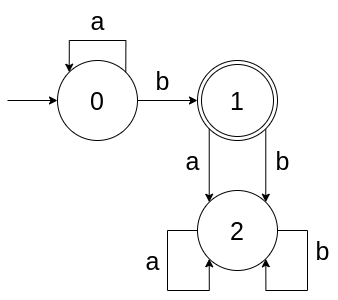
\includegraphics[width=0.4\textwidth, height=10cm,keepaspectratio]{chapters/chapter2/figures/Ejemplo 1 automatas.png}
    \caption{Caption}
    \label{fig:my_label}
\end{figure}

Los nodos 0 y 2 son nodos de no aceptación. EL nodo 1 es un nodo de aceptación. EL nodo inicial es el nodo 0. Este diagrama indica todas las posibles rutas o flujo de datos para definir si una cadena de caracteres cumple cierto patrón o no.

Es posible que varios autómatas puedan reconocer el mismo lenguaje. Si embargo es un problema indecidible encontrar el autómata mas eficiente que reconozca un lenguaje dado.

\subsubsection*{Ejemplo operadores relacionales}

\begin{figure}[H]
    \centering
    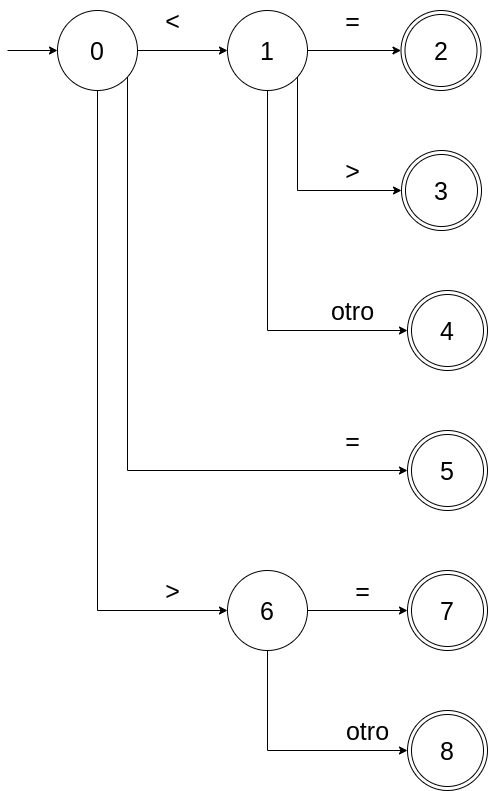
\includegraphics[width=0.5\textwidth, height=10cm,keepaspectratio]{chapters/chapter2/figures/Ejemplo 2 operadores relacionales.png}
    \caption{Caption}
    \label{fig:my_label}
\end{figure}

\subsection{Autómatas AFD}

Formalmente un autómata AFD(autómata finito determinista)se define como:
\begin{equation*}
    M=(\Sigma, Q, s, F, \delta)
\end{equation*}
donde 
\begin{itemize}
    \item $\Sigma$ es el alfabeto de entrada: $\Sigma=\{a_i\}_{i=1}^{i=n}$
    \item $Q$ es el conjunto de estados del autómata: $Q=\{q_j\}_{j=1}^{j=m}$
    \item $s$ es el estado inicial: $s\in Q$
    \item $F$ es el conjunto de estados de aceptación: $F \subseteq Q, F = \{q_r\}, F \neq \emptyset$
    \item $\delta$ es la función de transición: $\delta : Q\times\Sigma\rightarrow Q$, que significa que si el autómata esta en determinado estado, y lee un símbolo del alfabeto, entonces pase a un nuevo estado.
\end{itemize}

\subsubsection*{Ejemplo}

\begin{equation*}
    L=\{(ab)^i\vert i \geq 0\}
\end{equation*}
El lenguaje $L$ tiene asociado al menos un AFD:
\begin{enumerate}
    \item $\Sigma = \{a,b\},\: n=2$
    \item $Q=\{q_0, q_1, q_2\}$
    \item $s=q_0$
    \item $F=\{q_0\}$
    \item 
    \begin{tabular}{c|c|c}
         \Sigma & $a$ &$b$  \\ \hline
         $q_0$ & $q_1$ & $q_2$ \\ \hline
         $q_1$ & $q_2$ & $q_0$ \\ \hline
         $q_2$ & $q_2$ & $q_2$
    \end{tabular}
\end{enumerate}

Dado un lenguaje regular siempre es posible crear un AFD que lo reconozca

\subsection{Autómatas AFN}
Formalmente un autómata AFN(autómata finito no determinista) se define como:
\begin{equation*}
    M=(\Sigma, Q, s, F, \Delta)
\end{equation*}
donde 
\begin{itemize}
    \item $\Sigma$ es el alfabeto de entrada: $\Sigma=\{a_i\}_{i=1}^{i=n}$
    \item $Q$ es el conjunto de estados del autómata: $Q=\{q_j\}_{j=1}^{j=m}$
    \item $s$ es el estado inicial: $s\in Q$
    \item $F$ es el conjunto de estados de aceptación: $F \subseteq Q, F = \{q_r\}, F \neq \emptyset$
    \item $\Delta$ es la función de transición: $\Delta : Q\times\Sigma\rightarrow \mathcal {P}\{Q\}$ que mapea cada par de estados con símbolos en un subconjunto de $Q$
\end{itemize}

Los AFN se diferencian de los AFD en que $\Delta$ no es una función, sino una relación en la que dado u estado y un símbolo se puede ir a múltiples estados:
\begin{align*}
    \Delta:&Q\times\Sigma\rightarrow\mathcal {P}\{Q\}\\
    &(q_i, a_k)\rightarrow\Delta(q_i, a_k)
\end{align*}

\subsubsection*{Ejemplo}
Dado
\begin{enumerate}
    \item $\Sigma = \{a,b\},\: n=2$
    \item $Q=\{q_0, q_1, q_2, q_3, q_4\}$
    \item $s=q_0$
    \item $F=\{q_2, q_3, q_4\}$
    \item 
    \begin{tabular}{c|c|c}
         \Sigma & $a$ &$b$  \\ \hline
         $q_0$ & $\{q_1, q_4$\}$ & $\{q_3$\}$ \\ \hline
         $q_1$ & $\{q_1\}$ & $\{q_2\}$ \\ \hline
         $q_2$ & \emptyset & \emptyset \\ \hline
         $q_3$ & \emptyset & \emptyset \\ \hline
         $q_4$ & \emptyset & $\{q_4\}$
    \end{tabular}
\end{enumerate}

\subsection{Equivalencia}

Si $M$ es un autómata (AFD, AFM) y
\begin{equation*}
    L(M)=\{w\in\Sigma^*\vert\: w \text{ es aceptada por } M\}
\end{equation*}
donde $L$ es el lenguaje aceptado por $M$, entonces 
\begin{align*}
    &M_1, M2\text{ son autómatas (AFD, AFN)}\\
    & M_1 \sim M_2 \Longleftrightarrowhtarrow L(M_1) = L(M_2)
\end{align*}
Los autómatas $M_1$ y $M_2$ son equivalentes si aceptan el mismo lenguaje.
\subsection{Encontrar AFD quivalente a AFN}

Es posible implementar reconocedores de lenguajes usando AFN, sin embargo en un computador es mas sencillo y eficiente hacerlo mediante AFD. Es por estas razones que se realizan las transformaciones de AFN a AFD cuando se implementan reconocedores de tokens 

\subsubsection*{Teorema: Equivalencia entre AFN y un AFD}
Sea $M=(\Sigma, Q, s, F, \Delta)$, existe al menos un AFD $M'=(\Sigma, Q, s, F, \delta)$ que es equivalente a $M$
\subsubsection*{Demostración}
$M=(\Sigma, Q, s, F, \Delta)$\\
$M'=(\Sigma', Q', s', F', \delta)$

Defínase:
\begin{enumerate}
    \item $\Sigma'=\Sigma$
    \item $Q'=\mathbb{P}\{Q\}$
    \item $s'=\{s\}.\:s=q_0, s'=\{q_0\}\in Q'$
    \item $F'=\{q'\vert\:q'\in Q',\wedge.\exists_{x\in q'}x \in F\}$, es decir el conjunto de estados de $Q'$ que contengan al menos un estado de aceptación en $F$
    \item \begin{align*}
        \delta:&Q'\times\Sigma'\rightarrow Q'\\
        &(q',\alpha)\rightarrow\delta(q',\alpha)=\{P_1, P_2,\dots,P_m\}\\
        \text{donde:}&\\
        &\delta(q',\alpha)=\bigcup_{q\in q'}\Delta(q,\alpha)
    \end{align*} 
    
    
\end{enumerate}

\section{GENERADORES DE ANALIZADORES LÉXICOS: LEX}

Metalenguaje utilizado para la construcción de un analizador léxico. Tiene  como base la definición de categorías léxicas usando expresiones regulares. Flex es una nueva versión de LEX mas rápida (FAST LEX)

\begin{figure}[H]
    \centering
    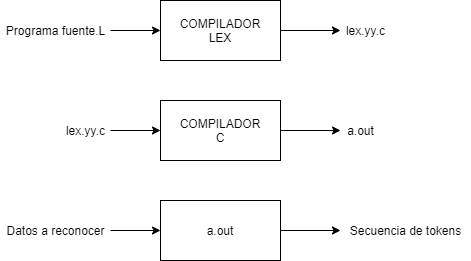
\includegraphics[width=0.8\textwidth, height=10cm,keepaspectratio]{chapters/chapter2/figures/Flex Funcionamiento.png}
    \caption{Funcionamiento Flex}
    \label{fig:my_label}
\end{figure}



\subsection{Expresiones regulares en LEX}

\begin{table}[H]
\begin{tabular}{c|c|c}
Expression                  & Matches                                & Example          \\ \hline
$c$                         & the one non-operator character $c$     & $a$              \\
$\backslash{}c$             & character $c$ literally                & $\backslash{}*$  \\
$"s"$                       & string $s$ literally                   & $"**"$           \\
$.$                         & any character but new line             & $a.*b$           \\
$\^{}$                      & begining of a line                     & $\^{}abc$        \\
$\$$                        & end of a line                          & $abc\$$          \\
$[s]$                       & any one of the characters in string $s$& $[abc]$          \\
$[\:\^{}s]$                 & any one character not in string $s$    & $[\:\^{}abc]$    \\
$r*$                        & zero or more strings matching $r$      & $a*$             \\
$r+$                        & one or more strings matching $r$       & $a+$             \\
$r?$                        & zero or one $r$                        & $a?$             \\
$r\{m,n\}$                  & between $m$ and $n$ ocurrences of $r$  & $a[1,5]$         \\
$r_1 \: r_2$                & an $r_1$ followed by an $r_2$          & $ab$             \\
$r_1 \vert r_2$             & an $r_1$ or an $r_2$                   & $a\vert b$       \\
$(r)$                       & same as $r$                            & $(a\vert b)$     \\
$r_1 / r_2$                 & $r_1$ when followed by $r_2$           & $abc/123$        \\
\end{tabular}
\end{table}

Existen otros metalenguajes para análisis léxico como AWK.\\


\subsection{Estructura de un programa en LEX}

Un programa en LEX consta de 3 partes, cada una separada por "\%\%":
\begin{enumerate}
    \item Es donde se escriben las declaraciones. Esta divida en 2 subsecciones. La primera escrita entre \%\{\dots\%\} se usa para escribir las variables manifiestas y otros elementos del código que con puestos literalmente en el código final. Después de ese limitador se escriben las extensiones regulares.
    \item Es donde se escriben las reglas de traducción. Esta estructurada en 2 partes: Una a la derecha llamada patrón y otra a la izquierda llamada acción. El patrón es escrito como una expresión regular, y la acción esta escrita entre llaves (\{, \}) y se escribe en lenguaje C. Cuando se detecta el patrón, se ejecuta la acción.
    \item Es donde se escriben las funciones auxiliares. Generalmente en las acciones definidas en la parte 2 se hacen llamados a funciones las cuales estarán definidas en esta sección.
\end{enumerate}

\subsection{Instalación}

Los repositorios del proyecto se encuentran en:
\begin{itemize}
    \item \verb|https://github.com/westes/flex|
    \item \verb|https://github.com/westes/flex/releases|
\end{itemize}

\subsubsection{Instalación en Windows}
\begin{itemize}
    \item \verb|http://gnuwin32.sourceforge.net/packages/flex.htm|
    \item \verb|http://gnuwin32.sourceforge.net/packages/bison.htm|
    \item \verb|https://sourceforge.net/projects/mingw/files|
\end{itemize}

\subsubsection{Instalación en Linux}
\begin{lstlisting}[language=shell]
sudo apt-get update
sudo apt-get install flex
\end{lstlisting}

\subsubsection{Ejecución}
\begin{lstlisting}[language=shell]
flex miarchivo.l
gcc lex.yy.c -lfl
\end{lstlisting}

\subsection{Devolución de valores}

Existe una función importante del analizador llamada \verb|int yylex()| que va a retornar el token que acaba de reconocer. \\
Existe una variable importante llamada \verb|char *yytext| que es un apuntador a la parte de la cadena donde se reconoció el patron.\\
Existe una variable llamada \verb|int yyval| donde se puede guardar inforamción para que sea usada despues. Ej:\\
\begin{lstlisting}[language=C]
[0-9]+      {yyval = atoi(yytext);}
\end{lstlisting}

\subsection{Comentarios y Entrada/Salida}

Los dispositivos de entrada y salida son los usuales: \verb|stdin()| y \verb|stdout()|, sin embargo si se  desea se pueden usar archivos utilizando la variable \verb|File *yyin|. Ej:\\
\begin{lstlisting}[language=C]
yyin = fopen("progr.py", "r");
\end{lstlisting}

También es posible escribir los resultados en un archivo usando la variable \verb|File *yyout|

\subsection{Ejemplos}
\subsubsection{Estructura de selección}

\begin{align*}
    sentencia \rightarrow & \: if\:\textbf{exp}\:then\:\textbf{sentencia}\\
    \vert & \: if\:\textbf{exp}\:then\:\textbf{sentencia}\:else\:\textbf{sentencia} \\
    \vert & \: \lambda\\
    exp \rightarrow & \: \textbf{term}\:relop\:\textbf{term}\\
    \vert & \: \textbf{term}\\
    term \rightarrow & \: id \\
    \vert & \: num
\end{align*}

Si este es el lenguaje entonces las categorías léxicas que surgen del son:

\begin{table}[H]
\begin{tabular}{c|c|c}
Regular Expression & Token & Attribute-Value\\ \hline
ws & - & - \\
if & if & - \\
then & then & - \\
else & else & - \\
id & id & pointer to table entry \\
num & num & pointer to table entry \\
\textless & relop & LT \\
\textless = & relop & LE \\
= & relop & EQ \\
\textless\textgreater & relop & NE \\
\textgreater & relop & GT \\
\textgreater= & relop & GE \\
\end{tabular}
\end{table}

Después de eso, se construyen las expresiones regulares para cada categoría:

\begin{align*}
    digito \rightarrow & \: [0-9]\\
    digitos \rightarrow & \: digito+\\
    numero \rightarrow & \: digitos(.\:digitos)?(E[+\:-]?\:digitos)?\\
    letra \rightarrow & \: [a-zA-Z]\\
    id \rightarrow & \: letra(letra\vert digito)*\\
    if \rightarrow & \: if\\
    then \rightarrow & \: then\\
    else \rightarrow & \: else\\
    relop \rightarrow & \: \textless\vert\textgreater\vert\textless=\vert\textgreater=\vert=\vert\textless\textgreater \\
\end{align*}

Esto nos lleva al ejemplo (tomado del libro de Aho):
\begin{lstlisting}[language=C]
%{
    \* Definitions of manifest constants
    LT, LS, EQ, WE, GT, GE,
    IF, THEN, ELSE, ID, NUMBER, RELOP */
%}
/* regular definitions */
delim       [ \t\n]
ws          {delim}+
letter      [A-Za-z]
digit       [0-9]
id          {letter}({letter}|{digit})*
number      {digit}+(\.{digit}+)?(E[+-]?{digit}+)?

%%

{ws}        {/* no action and no return */}
if          {return(IF);}
then        {return(THEN);}
else        {return(ELSE);}
{id}        {yyval = (int) installID(); return(ID);}
{number}    {yyval = (int) installNum(); return(NUMBER);}
"<"         {yyval = LT; return(RELOP);}
"<="        {yyval = LE; return(RELOP);}
"="         {yyval = EQ; return(RELOP);}
"<>"        {yyval = NE; return(RELOP);}
">"         {yyval = GT; return(RELOP);}
">="        {yyval = GE; return(RELOP);}

%%

int installID(){
    /* function to install the lexemes, whose
    first character is pointed by yytext,
    and whose length is yyleng, into the
    symbol table and return a pointer 
    thereto */
}

int installNum(){
    /* similar to instalID, but puts
    numerical constants into a separate table */
}

\end{lstlisting}



\section{EJERCICIOS DEL CAPÍTULO}
\begin{enumerate}
    \item Demostrar el Teorema 2 (Sugerencia: Diagonalización)
    \item Dado $\Sigma=\{a, b\}$, verificar que el lenguaje $L=\{(ab)^i|i \geq 0\}$ es un lenguaje regular
    \item Escribir formalmente el lenguaje de todas las cadenas que no contienen ninguna sub-cadena $ac$ cuando $\Sigma=\{a,b,c\}$
    \begin{enumerate}
        \item Mostrarlo
        \item Verificar que es regular
        \item Proponer sobre el mismo alfabeto un lenguaje que no sea regular
    \end{enumerate}
    \item Demostrar que la distancia de Damerau-Levenshtein cumple con las 5 condiciones para ser una distancia
    \item Análisis, diseño e implementación de un programa en lenguaje R que permita
    \begin{enumerate}
        \item Recibir el vocabulario de un lenguaje de programación(JAVA, C++, C#) y calcule la distancia de Damerau-Levenshtein de sis palabras
        \item Obtener el histograma del lenguaje
        \item Calcular la distancia promedio y la varianza
        \item Proponer una distancia entre lenguajes
    \end{enumerate}
    \item Análisis, diseño e implemencación de un programa en GO que:
    \begin{enumerate}
        \item Reciba una matriz de números enteros $A$ de tamaño $n\times m$ y obtenga como resultado su matriz inversa generalizada de Moore-Penrose.
        \item Las operaciones de multiplicación de números enteros involucradas en el calculo deben usar el algoritmo inventado por los científicos A. A. Karatsubay Y. Ofman
    \end{enumerate}
    \item Escribir el lenguaje reconocido por la expresión regular $a|a^*b$ donde $\Sigma=\{a, b\}$
    \item Demostrar la 12 ley algebraica de las expresiones regulares ($(r^*s)^*=\lambda|(r|s)^*$)
    \item Realizar una definición regular que reconozca números complejos. \item Usando extinciones regulares, escribir la definición regular para números reales sin signo
    \item Completar e implementar en FLEX el ejemplo de la sección 3.5.6.1
    \item Un estadístico (profesional que trabaja en el campo de la estadística matemática) ha contratado a su grupo de trabajo para que le ayuden a construir un lenguaje de programación de propósito especifico para el problema de dos vías de clasificación. en el cual desea experimentar con diversas estadísticas pertenecientes al conjunto de pruebas de Friedman. En la primera etapa ustedes se comprometen a:
    \begin{enumerate}
        \item Definir las categorías léxicas necesarias y el vocabulario completo para la construcción de ese lenguaje de propósito específico.
        \item Especificar los patrones basados en expresiones regulares, definiciones regulares y extensiones regulares para las diferentes categorías léxicas que ustedes han propuesto
        \item Construir el analizador léxico en el lenguaje de programación C para este lenguaje de programación utilizando el metalenguaje FLEX.
    \end{enumerate}
    \item Crear el diagrama de transición de un AFD que reconozca números complejos
    \item Dado el autómata:
    \begin{enumerate}
        \item $\Sigma=\{a,b\}$
        \item $Q=\{q_0, q_1\}$
        \item $s=q_0$
        \item $F = \{q_0\}$
        \item 
        \begin{tabular}{c|c|c}
         \Sigma & $a$ &$b$  \\ \hline
         $q_0$ & $q_0$ & $q_1$ \\ \hline
         $q_1$ & $q_1$ & $q_0$
    \end{tabular}
    \end{enumerate}
    Encontrar el lenguaje aceptado por el autómata, y encontrar la expresión regular asociada.
    \item Dado el autómata:
    \begin{enumerate}
        \item $\Sigma=\{a,b\}$
        \item $Q=\{q_0, q_1, q_2, q_3\}$
        \item $s=q_0$
        \item $F = \{q_0, q_1, q_2\}$
        \item 
        \begin{tabular}{c|c|c}
         \Sigma & $a$ &$b$  \\ \hline 
         $q_0$ & $q_0$ & $q_1$ \\ \hline
         $q_1$ & $q_0$ & $q_2$ \\ \hline
         $q_2$ & $q_0$ & $q_3$ \\ \hline
         $q_3$ & $q_3$ & $q_3$
    \end{tabular}
    \end{enumerate}
    Encontrar la expresión regular del lenguaje que ese autómata reconoce
\end{enumerate}
